\documentclass[12pt,twoside, a4paper, twocolumn]{article}
\usepackage[utf8]{inputenc}
\usepackage[brazil]{babel}
\usepackage[margin = 0.5in]{geometry}
\usepackage{amsmath}
\usepackage{amsthm}
\usepackage{amssymb}
\usepackage{amsthm}
\usepackage{setspace}
\usepackage[americanvoltages,fulldiodes,siunitx]{circuitikz}
\usepackage{lipsum}
\usepackage{pgfplots}
\usepackage{ifthen}
\usepackage{adjustbox}
\usepackage[section]{placeins}
\usepackage{hyperref}
\usepackage{graphicx}
\usepackage{amsmath}
\usepackage{amsthm}
\usepackage{amssymb}
\usepackage{amsthm}
\usepackage{setspace}
\usepackage[americanvoltages,fulldiodes,siunitx]{circuitikz}
\usepackage{lipsum}
\usepackage{pgfplots}
\usepackage{ifthen}
\usepackage{adjustbox}
\usepackage[section]{placeins}
\usepackage{hyperref}
\usepackage{graphicx}
\usepackage{adjustbox}
\usepackage{indentfirst}








\pgfplotsset{compat=newest}
\graphicspath{ {./images/} }
%  #1 color - optional #2 x_0 #3 y_0 #4 x_f #5 y_f #6 name - optional  #7 true if adding lines to axis
\newcommand{\drawvector} [9] [color=cyan] {
\draw[line width=1.5pt,#1,-stealth](axis cs: #2, #3)--(axis cs: #4, #5) node[anchor=south west]{$#6$};
\ifthenelse{\equal{#7}{true}}{
\draw[line width=1pt,#1, dashed](axis cs: #4, #5)--(axis cs: #4, 0) node[anchor= north west]{$#8$};
\draw[line width=1pt,#1, dashed](axis cs: #4, #5)--(axis cs: 0, #5) node[anchor=south east]{$#9$};
}
{}
}
\newcommand\deriv[2]{\frac{\mathrm d #1}{\mathrm d #2}}
\title{Sétimo Relatório de Lab de Circuitos II}
\author{Henrique da Silva \\ hpsilva@proton.me}
\date{\today}
\pgfplotsset{width = 10cm, compat = 1.9}
\begin{document}
\maketitle
\pagenumbering{gobble}
\newpage
%pagenumbering{roman}
\tableofcontents
\newpage




\section{Introdução}




Neste relatório, vamos discutir quadripolos, e vamos projetar, montar e testar um quadripolo em cascata, obtendo seus parâmetros \emph{a}.








Todos arquivos utilizados para criar este relatório, e o relatorio em si estão em:  \url{https://github.com/Shapis/ufpe_ee/tree/main/5th semester/Circuits II/}




\section{Análise preliminar}




Utilizarei o Maxima para fazer a análise teórica do circuito antes de montá-lo fisicamente.


Após terminar as análises compararei os resultados obtidos nas análises numéricas e em laboratório para verificar sua coerência.




\subsection{Os circuitos}


Vamos utilizar dois circuitos em cascata, o quadripolo "A" e o quadripolo "B", ambos puramente resistivos e representados abaixo.




\begin{figure}[h]
    \centering
    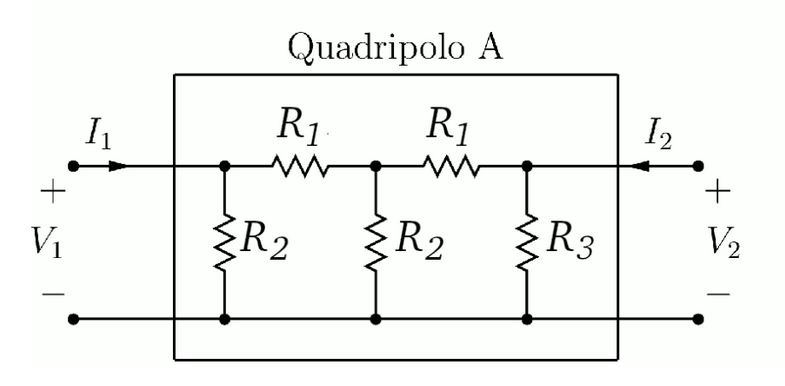
\includegraphics[width=1\columnwidth]{images/quadripoloa.png}
    \caption{Quadripolo "A" puramente resistivo.}
\end{figure}


\begin{figure}[h]
    \centering
    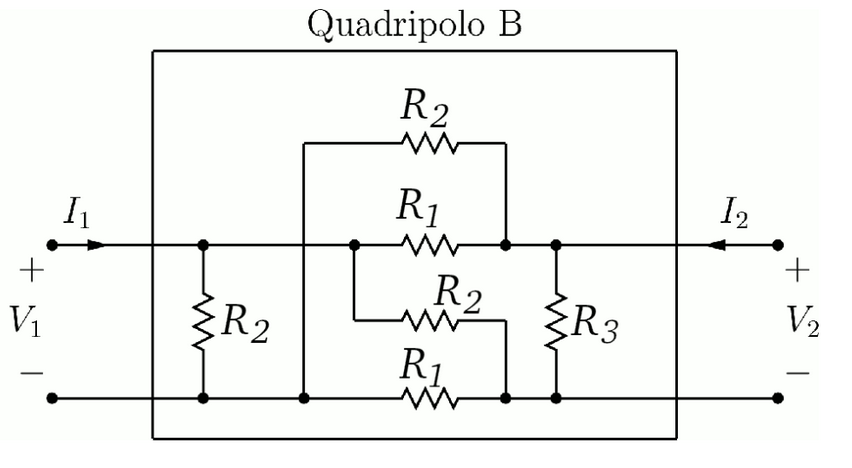
\includegraphics[width=1\columnwidth]{images/quadripolob.png}
    \caption{Quadripolo "B" puramente resistivo.}
\end{figure}




\pagebreak
\subsection{Maxima}




Podemos realizar a análise dos quadripolos acima utilizando análise nodal.


\subsubsection{Quadripolo \emph{A}}


\begin{equation}
    \begin{aligned}
         & {{V_{1}-{\it Va}}\over{R_{1}}}+{{V_{1}}\over{R_{2}}}-I_{1}=0                              \\
         & {{{\it Va}-V_{2}}\over{R_{1}}}+{{{\it Va}-V_{1}}\over{R_{1}}}+{{ {\it Va}}\over{R_{2}}}=0 \\
         & {{V_{2}-{\it Va}}\over{R_{1}}}+{{V_{2}}\over{R_{3}}}-I_{2}=0
    \end{aligned}
\end{equation}


\subsubsection{Quadripolo \emph{B}}


\begin{equation}
    \begin{aligned}
         & {{V_{1}-{\it Vb}}\over{R_{2}}}+{{V_{1}-{\it Va}}\over{R_{1}}}+{{ V_{1}}\over{R_{2}}}-I_{1}=0       \\
         & {{{\it Va}-{\it Vb}}\over{R_{3}}}+{{{\it Va}-V_{1}}\over{R_{1}}}+{{ {\it Va}}\over{R_{2}}}-I_{2}=0 \\
         & {{{\it Vb}-{\it Va}}\over{R_{3}}}+{{{\it Vb}-V_{1}}\over{R_{2}}}+{{ {\it Vb}}\over{R_{1}}}+I_{2}=0 \\
         & V_{2}={\it Va}-{\it Vb}
    \end{aligned}
\end{equation}


\subsubsection{Parámetros "y" do quadripolo \emph{B}}


Resolvendo as quatro equações acima para $I_1$, $I_2$, $V_1$ e $V_2$ obtemos:


\begin{equation}
    \begin{aligned}
         & I_{1}={{-R_{2}\,V_{2}+R_{1}\,V_{2}+\left(R_{2}+3\,R_{1}\right)\, V_{1}}\over{2\,R_{1}\,R_{2}}}                                                                \\
         & I_{2}=-{{R_{2}\,\left(-R_{3}\,V_{2}-2\,R_{1}\,V_{2}\right)-R_{1}\, R_{3}\,V_{2}+\left(R_{2}\,R_{3}-R_{1}\,R_{3}\right)\,V_{1}}\over{2\, R_{1}\,R_{2}\,R_{3}}} \\
         & {\it Va}={{V_{2}+V_{1}}\over{2}}                                                                                                                              \\
         & {\it Vb}={{V_{1}-V_{2}}\over{2}}
    \end{aligned}
\end{equation}


Com estes em mãos podemos calcular a solução simbólica dos parâmetros \emph{y}.


Fazendo $V_2 = 0$:


\begin{equation}
    \begin{aligned}
         & y11 = {{R_{2}+3\,R_{1}}\over{2\,R_{1}\,R_{2}}}                    \\
         & y21 = -{{R_{2}\,R_{3}-R_{1}\,R_{3}}\over{2\,R_{1}\,R_{2}\,R_{3}}}
    \end{aligned}
\end{equation}


Fazendo $V_1 = 0$


\begin{equation}
    \begin{aligned}
         & y12 = {{R_{1}\,V_{2}-R_{2}\,V_{2}}\over{2\,R_{1}\,R_{2}\,V_{2}}}                                                      \\
         & y22 = -{{R_{2}\,\left(-R_{3}\,V_{2}-2\,R_{1}\,V_{2}\right)-R_{1}\,R_{3}\, V_{2}}\over{2\,R_{1}\,R_{2}\,R_{3}\,V_{2}}}
    \end{aligned}
\end{equation}


E para conseguir a solução numérica, basta substituir $R_1$, $R_2$, e $R_3$ pelos valores dos resistores que desejamos.


No caso:


\begin{equation}
    \begin{aligned}
         & R_1 = 8.2k \varOmega \\
         & R_2 = 47k \varOmega  \\
         & R_3 = 82k \varOmega  \\
    \end{aligned}
\end{equation}


Que nos dá os seguintes parâmetros \emph{y}:


\begin{equation}
    \begin{aligned}
         & y11 = 9.289050337311884 \times 10^{-5}  \\
         & y12 = -5.033731188375714 \times 10^{-5} \\
         & y21 = -5.033731188375714 \times 10^{-5} \\
         & y22 = 8.38090295796575 \times 10^{-5}   \\
    \end{aligned}
\end{equation}


\subsubsection{Impedância de  entrada com carga}


Aqui introduziremos uma carga $Z_L = 2k \varOmega$ na saída do quadripolo \emph{B}, e analisaremos o que ocorre com sua impedância de entrada. Ou seja. Com $\frac{V_1}{I_1}.$


\begin{equation}
    \begin{aligned}
         & I_1 = 9.2890 10^{-5} V_1 + -5.0337 10^{-5} V_2 \\
         & I_2 = -5.0337 10^{-5} V_1 + 8.3809 10^{-5} V_2 \\
    \end{aligned}
\end{equation}


E aqui conectamos a carga $Z_L$ a saída do quadripolo fazendo $V_2 = -I_2 Z_L$:


\begin{equation}
    \begin{aligned}
         & I_1 = 9.2890 10^{-5} V_1 + -5.0337 10^{-5}  (-2000 I_2) \\
         & I_2 = -5.0337 10^{-5} V_1 + 8.3809 10^{-5} (-2000 I_2)  \\
    \end{aligned}
\end{equation}


\paragraph*{}
\paragraph*{}
\paragraph*{}
\paragraph*{}
Daqui resolvemos para $V_1$, $V_2$ e $I_2$ e obtemos a impedância de entrada com a carga:


\begin{equation}
    \frac{V_1}{I_1} = 11293.0154298157 \varOmega
\end{equation}


\subsubsection{Parâmetros \emph{a} do quadripolo em cascata}


A análise do quadripolo \emph{A} foi realizada no relatório 6. Então pegarei os seus parâmetros \emph{z} previamente obtidos para realizar a análise do quadripolo em cascata.


\begin{equation}
    \begin{aligned}
         & z_{11} = 21343.61254363896 \\
         & z_{12} = 15333.99250307293 \\
         & z_{21} = 15333.99250307293 \\
         & z_{22} = 23826.62255647245 \\
    \end{aligned}
\end{equation}


Podemos convertê-los para parâmetros \emph{a} do quadripolo $"A"$ com as seguintes operações:




\begin{equation}
    \begin{aligned}
         & a_{11} = \frac{z_{11}}{z_{21}} = 1.391914893617021      \\
         & a_{12} = \frac{\varDelta z}{z_{21}} = 17830.63829787234 \\
         & a_{21} = \frac{1}{z_{21}} = 6.521458777285825 * 10^-5   \\
         & a_{22} = \frac{z_{22}}{z_{21}} = 1.553843368039837
    \end{aligned}
\end{equation}


E convertemos os parâmetros \emph{y} do quadripolo $"B"$ da seguinte forma:


\begin{equation}
    \begin{aligned}
         & a_{11} = -\frac{y_{22}}{y_{21}} = 1.664948453608247              \\
         & a_{12} = -\frac{1}{y_{21}} = 19865.9793814433                    \\
         & a_{21} = -\frac{\varDelta y}{y_{21}} = 1.043205880622088 * 10^-4 \\
         & a_{22} = -\frac{y_{11}}{y_{21}} = 1.845360824742268
    \end{aligned}
\end{equation}


Agora para achar os parâmetros \emph{a} do quadripolo em cascata, basta fazer a multiplicação matricial dos parâmetros \emph{a} de cada quadripolo.


E isto nos dará os seguintes resultados para parâmetro \emph{a} do quadripolo em cascata:


\begin{equation}
    \begin{aligned}
         & a_{11} = 4.177569222440531       \\
         & a_{12} = 60555.71397236235       \\
         & a_{21} = 2.706767809755985*10^-4 \\
         & a_{22} = 4.162953335231222
    \end{aligned}
\end{equation}


\subsubsection{Equações parâmetro \emph{a} em cascata}


Agora que temos os parâmetros \emph{a} do quadripolo em cascata, podemos escrever as equações que relacionam as tensões e correntes de entrada e saída do quadripolo em cascata.


\begin{equation}
    \begin{aligned}
         & V_1 = a_{11} V_2 - a_{12} I_2 \\
         & I_1 = a_{21} V_2 - a_{22} I_2 \\
    \end{aligned}
\end{equation}


Substituindo pelos valores achados temos:


\begin{equation}
    \begin{aligned}
         & V_1 = 4.1775 V_2 - 60555.71 I_2    \\
         & I_1 = 2.7 * 10^-4 * V_2 - 4.16 I_2 \\
    \end{aligned}
\end{equation}


Para achar a impedância de entrada com uma carga resistiva de $2k \varOmega$ fazemos novamente  $V_2 = -I_2 Z_L$:


\begin{equation}
    \begin{aligned}
         & V_1 = 4.1775 V_2 - 60555.71 (-2000 I_2)    \\
         & I_1 = 2.7 * 10^-4 * V_2 - 4.16 (-2000 I_2) \\
    \end{aligned}
\end{equation}


E resolvemos para $V_1$, $V_2$, e $I_2$.


Com isto em mãos temos:


\begin{equation}
    \frac{V_1}{I_1} = 14648.46021387691 \varOmega
\end{equation}




\section{Medições em laboratório}


Inicialmente farei as medições dos componentes a serem usados.


Após isso montarei os circuitos e realizei as medições de tensão e corrente de ambos quadripolos e da conexão em cascata, com estes obterei os parâmetros \emph{z} do quadripolo A e os parâmetros \emph{y} do quadripolo B, e parâmetros \emph{a} do quadripolo em cascata.


E por fim, medir a impedância total do circuito para confirmar que os resultados que obtive são coerentes




\subsection{Quadripolo A}


\subsubsection{Tabela de medidas}
\begin{equation}
    \begin{aligned}
        R_{11} & = 8.22k \varOmega  \\
        R_{12} & = 8.217k \varOmega \\
        R_{21} & = 46.53k \varOmega \\
        R_{22} & = 46.34k \varOmega \\
        R_{3}  & = 82.05k \varOmega \\
        Z_L    & = 1.9475 \varOmega
    \end{aligned}
\end{equation}


\subsubsection{Resultados das medidas}


\begin{center}
    \begin{tabular}{ |c|c|c| }
        \hline
        $V_1$ & $0.643 V$     & $1.0082 V$    \\
        $V_2$ & $1.005 V$     & $0.7215 V$    \\
        $I_1$ & $0$           & $47.33 \mu A$ \\
        $I_2$ & $42.18 \mu A$ & $0$           \\
        \hline
    \end{tabular}
\end{center}


\subsubsection{Parâmetros \emph{z}}


Para $I_1 = 0$:


\begin{equation}
    \begin{aligned}
         & z_{12} = \frac{V_1}{I_2} =  15244.19156 \varOmega \\
         & z_{22} = \frac{V_2}{I_2} = 23826.458037 \varOmega \\
    \end{aligned}
\end{equation}


Para $I_2 = 0$:


\begin{equation}
    \begin{aligned}
         & z_{11} = \frac{V_1}{I_1} = 21301.5001056 \varOmega \\
         & z_{21} = \frac{V_2}{I_1} = 15244.0312698 \varOmega
    \end{aligned}
\end{equation}


E assim podemos montar as equações para parâmetro \emph{z}:


\begin{equation}
    \begin{aligned}
         & V_1 = 21301.5 I_1 + 15244.19 I_2  \\
         & V_2 = 15244.03 I_1 + 23826.45 I_2 \\
    \end{aligned}
\end{equation}


\subsubsection{Impedância de entrada com carga}


Novamente podemos substituir $I_2 = -I_1 Z_L$ que nos dá:


\begin{equation}
    \begin{aligned}
         & Z_{numerico} = 11547.1061332794 \varOmega \\
         & Z_{experimental} = 12204 \varOmega
    \end{aligned}
\end{equation}


Observamos que o valor da impedância obtido numericamente a partir dos parâmetros \emph{z} é bastante próximo do valor obtido experimentalmente.




\subsection{Quadripolo B}


\subsubsection{Tabela de medidas}
\begin{equation}
    \begin{aligned}
        R_{11} & = 8.188k \varOmega \\
        R_{12} & = 8.188k \varOmega \\
        R_{21} & = 46.05k \varOmega \\
        R_{22} & = 46.92k \varOmega \\
        R_{23} & = 46.79k \varOmega \\
        R_{3}  & = 81.74k \varOmega \\
        Z_L    & = 1.9475 \varOmega
    \end{aligned}
\end{equation}


\subsubsection{Resultados das medidas}


\begin{center}
    \begin{tabular}{ |c|c|c| }
        \hline
        $V_1$ & $0 V$          & $1.0036 V$     \\
        $V_2$ & $1.003 V$      & $0 V$          \\
        $I_1$ & $0.12 \mu$     & $162.62 \mu A$ \\
        $I_2$ & $153.66 \mu A$ & $0.13 \mu$     \\
        \hline
    \end{tabular}
\end{center}


\subsubsection{Parâmetros \emph{y}}


Para $V_1 = 0$:


\begin{equation}
    \begin{aligned}
         & y_{12} = \frac{I_1}{V_2} =  -1.19641077 * 10^-7 \sigma \\
         & y_{22} = \frac{I_2}{V_2} = 1.53 * 10^-4 \sigma         \\
    \end{aligned}
\end{equation}


Para $V_2 = 0$:


\begin{equation}
    \begin{aligned}
         & y_{11} = \frac{I_1}{V_1} = 1.62 * 10^-4 \sigma  \\
         & y_{21} = \frac{I_2}{V_1} = -1.29 * 10^-7 \sigma
    \end{aligned}
\end{equation}


Observo que os resultados não estão coerentes com as análises teóricas. Creio que o problema foi na medição das correntes. As medições estavam flutuando dependendo do momento que as fiz. E não tenho certeza do por quê.


Mas vou prosseguir a análise, mesmo com os parâmetros \emph{y} incoerentes.


\begin{equation}
    \begin{aligned}
         & I_1 = 1.62 * 10^-4 * V_1 -1.19641077 * 10^-7 V_2 \\
         & I_2 = -1.29 * 10^-7 *  V_1 + 1.53 * 10^-4 V_2    \\
    \end{aligned}
\end{equation}


\subsubsection{Impedância de entrada com carga}


Novamente podemos substituir $I_2 = -I_1 Z_L$ que nos dá:


\begin{equation}
    \begin{aligned}
         & Z_{numerico} = 6172.838067895077 \varOmega \\
         & Z_{experimental} = 7000 \varOmega
    \end{aligned}
\end{equation}


Estou deveras confuso de por que os resultados foram próximos. Quando os parametros \emph{y} numericos e experimentais estavam tão distantes. Coincidência? Ou interpretei mal o resultado numérico e experimental?


\subsection{Quadripolo em cascata}


\subsubsection{Tabela de medidas}


Utilizaremos os mesmos componentes  dos quadripolos A e B, logo serão as mesmas respectivas tabelas listadas acima.


\subsubsection{Resultados das medidas}


\begin{center}
    \begin{tabular}{ |c|c|c| }
        \hline
        $V_1$ & $1.003V$   & $1.003 V$     \\
        $V_2$ & $0.2982 V$ & $0 V$         \\
        $I_1$ & $65.8 \mu$ & $74.06 \mu A$ \\
        $I_2$ & $0$        & $0.1 \mu$     \\
        \hline
    \end{tabular}
\end{center}


\subsubsection{Parâmetros \emph{a}}


Para $V_2 = 0$:


\begin{equation}
    \begin{aligned}
         & a_{12} = -\frac{V_1}{I_2} =  1 * 10^8 \varOmega \\
         & a_{22} = \frac{I_1}{I_2} = 740.6                \\
    \end{aligned}
\end{equation}


Para $I_2 = 0$:


\begin{equation}
    \begin{aligned}
         & a_{11} = \frac{V_1}{V_2} = 3.36351441985         \\
         & a_{21} = \frac{I_1}{V_2} = 2.2 * 10^-4 \varOmega
    \end{aligned}
\end{equation}


Novamente observo que os resultados não estão coerentes com as análises teóricas. Creio que o problema foi na medição das correntes. As medições estavam flutuando dependendo do momento que as fiz. E não tenho certeza do por quê.


Mas vou prosseguir a análise, mesmo com os parâmetros \emph{a} incoerentes.


\begin{equation}
    \begin{aligned}
         & V_1 = 3.36351441985 * V_2 -  10^8 I_2 \\
         & I_1 = 2.2 * 10^-4 *  V_2 + 740.6  I_2 \\
    \end{aligned}
\end{equation}


\subsubsection{Impedância de entrada com carga}


Novamente podemos substituir $I_2 = -I_1 Z_L$ que nos dá:


\begin{equation}
    \begin{aligned}
         & Z_{numerico} = -135090.0570605898 \varOmega \\
         & Z_{experimental} = 13683 \varOmega
    \end{aligned}
\end{equation}


O resultado numérico com os parâmetros \emph{a} obtidos foi bastante incoerente. Creio que por erros de medição das correntes do circuito. Mas o resultado experimental foi bastante próximo do esperado.




\section{Conclusões}


Conseguimos com sucesso fazer a análise numérica pelo Maxima, e comparamos os resultados com os obtidos experimentalmente.




Nos resultados práticos, obtivemos parâmetros $Z$ bastante similares aos obtidos numericamente.


Porém para os parâmetros $y$ e $a$ eles foram incoerentes. Imagino que houve algum erro no quadripolo $B$, que propagou-se para o quadripolo em cascata.


As impedâncias de entrada com a carga $Z_L$ experimentais foram coerentes com a análise numérica em todos casos.


Em suma creio que conseguimos entender melhor como fazer análise de quadripolos, apesar de ter errado nas medições das correntes do quadripolo $B$, e não ter identificado o erro a tempo de corrigi-lo.




\end{document}